\documentclass[border=2pt]{standalone}
\usepackage{tikz}
\usepackage{relsize,bm}
\begin{document}
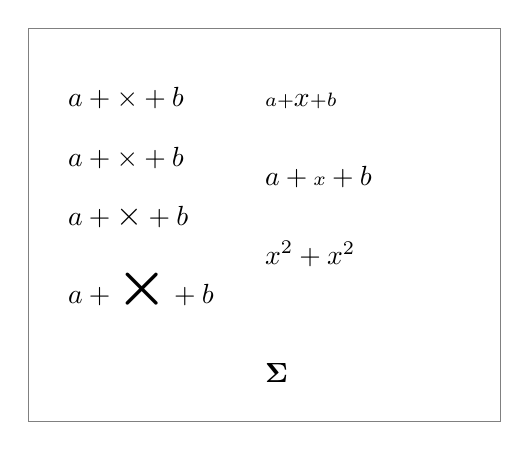
\begin{tikzpicture}
  \draw[gray] (0,-4) rectangle (6,1);
  \node[anchor=base west,inner sep=0pt] at (.5,0) {$a+\times+b$};
  \node[anchor=base west,inner sep=0pt] at (.5,-.75) {$a+\mathlarger{\times}+b$};
  \node[anchor=base west,inner sep=0pt] at (.5,-1.5) {$a+\mathlarger{\mathlarger{\times}}+b$};
  \node[anchor=base west,inner sep=0pt] at (.5,-2.5) {$a+\mathlarger{\mathlarger{\mathlarger{\mathlarger{\mathlarger{\bm{\times}}}}}}+b$};
  \node[anchor=base west,inner sep=0pt] at (3,0) {$\scriptstyle a+\mathlarger{x}+b$};
  \node[anchor=base west,inner sep=0pt] at (3,-1) {$a+\mathsmaller{x}+b$};
  \node[anchor=base west,inner sep=0pt] at (3,-2) {$\mathlarger{x^2}+x^2$};
  \node[anchor=base west,inner sep=0pt] at (3,-3.5) {$\boldsymbol\Sigma$};
\end{tikzpicture}
\end{document}
